\chapter{正则系综和广义系综} % (fold)
\label{cha:正则系综和广义系综}
\section{正则系综} % (fold)
\label{sec:正则系综}
\subsection{正则系综和配分函数} % (fold)
\label{sub:正则系综和配分函数}
所谓正则系综,就是固定了$N,V,T$作为状态参量的系综。一般来说,我们可以将正则系综看作微正则系综的一个子系统。让正则系综与热库\index{热库}接触(reservoir)。当正则系综和环境达到热平衡的时候,两者就构成了一个微正则系综。
\begin{figure}[h]
       \centering
       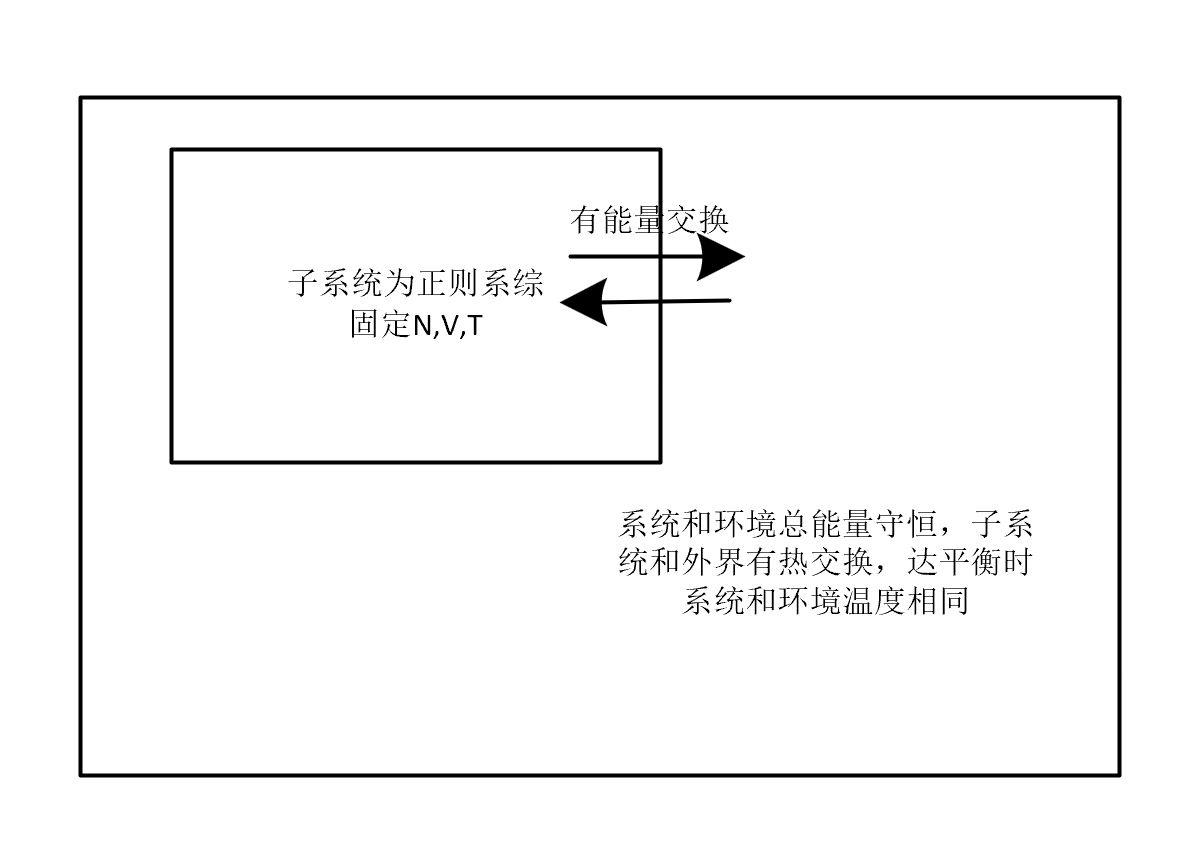
\includegraphics[width=0.45\textwidth]{fig/正则系综.png}
       \caption{正则系综}
\end{figure}

系统和环境的总能量是一个定值\begin{equation}
       E_{sys}+E_{envir}=E_0
\end{equation}
所以$E_{envir}=E_0-E_{sys}$,考虑系统处于能量$E_{sys}$时的概率,显然,应该正比于这个时刻系统和环境的状态数之积
\begin{equation}
       p(E_{sys})\propto \Omega_{sys}(E_{sys})\Omega(E_{0}-E_{sys})
\end{equation}
我们可以直接考虑系统处于某一个状态的概率,于是\begin{equation}
\begin{aligned}
       p(E_{sys})&\propto \Omega(E_{0}-E_{sys})\\
       &=e^{\ln \Omega(E_{0}-E_{sys})}
\end{aligned}
\end{equation}
假设$E_0\ll E_{sys}$,因此
\begin{equation}
       \ln \Omega(E_{0}-E_{sys})=\ln \Omega(E_0)-E_{sys} \left.\diffp{\Omega}{E}\right|_{E=E_0}
\end{equation}
\begin{definition}
       定义\begin{equation}
              \beta=\left.\diffp{\Omega}{E}\right|_{E=E_0}
       \end{equation}
\end{definition}
因为对于微正则系综$E_0$是一个常数,因此$\Omega(E_0)$也是一个常数,所以\begin{equation}
       p\propto e^{-\beta E_{sys}}
\end{equation}
归一化之后可以得到\begin{equation}
       p_i =\frac{\displaystyle e^{-\beta E_{sys}}}{\displaystyle \sum e^{-\beta E_{sys}}}
\end{equation}其中,求和是对所有可能的状态求和。

\begin{definition}
       我们记\begin{equation}
              Q=\sum e^{-\beta E_{sys}(N,V)}=Q(N,V,T)
       \end{equation}
       为系统的配分函数\index{配分函数}。
\end{definition}

当然,对系统的所有状态的求和也可以变换成对能级的求和\begin{equation}
      \begin{aligned}
       Q&=\sum e^{-\beta E_{sys}(N,V)}=\sum_{E}\Omega(E) e^{-\beta E}\\
       &=\int_0^{+\infty} \overline{\Omega}(E) e^{-\beta E} \di E 
      \end{aligned} 
\end{equation}
从上式我们不难发现正则配分函数就是对微正则系综中的态密度函数做了一个Laplace变换,这也反映了两者的等价性。
% subsection 正则系综和配分函数 (end)
\subsection{均值、涨落和能量的正则分布} % (fold)
\label{sub:均值、涨落和能量的正则分布}
首先我们来考虑能量的均值\index{均值}
\begin{equation}
\begin{aligned}
       \braket{E}&=\sum_{v}p_v E_v =\sum_{v}\frac{e^{-\beta E_v}E_v}{Q}\\
       &=-\diffp*{\ln Q}{\beta}{N,V}\label{equ:energy mean in canolical ensemble}
\end{aligned}
\end{equation}

然后我们就可以来考虑能量的涨落\index{涨落}
\begin{equation}
       \braket{(\Delta E)^2}=\braket{E^2}-\braket{E}^2
\end{equation}
对于$\braket{E^2}$,我们有\begin{equation}
\begin{aligned}
       \braket{E^2}&=\sum_{v}p_v E_v^2 =\sum_{v}\frac{e^{-\beta E_v}E_v^2}{Q}\\
       &=\frac{1}{Q} \diffp[2]{Q}{\beta}\\
\end{aligned}
\end{equation}
因此\begin{equation}
       \begin{aligned}
              \Delta ^2 &=\braket{E^2}-\braket{E}^2=\frac{1}{Q} \diffp[2]{Q}{\beta}-\frac{1}{Q^2} \left(\diffp[1]{Q}{\beta}\right)^2\\
       &=\diffp{}{\beta} \left(\frac{1}{Q} \diffp{Q}{{\beta}}\right)\\
       &=-\diffp{{\braket{E}}}{\beta}
       \end{aligned}
\end{equation}

\begin{remark}
       一个有用的微分关系:\begin{equation}
              \diffp{}{\beta} =\diffp{}{T} \diffp{T}{\beta}=-kT^2 \diffp{}{T}
       \end{equation}
\end{remark}

因此就有了\begin{equation}
              \braket{(\Delta E)^2} =\diffp{{\braket{E}}}{\beta}=kT^2 \diffp{\braket{E}}{T} =kT^2 C_V
\end{equation}

\begin{definition}
       定义涨落的相对值\index{相对涨落}为\begin{equation}
              \sigma_E=\frac{\sqrt{\braket{(\Delta E)^2}}}{\braket{E}}=\frac{\sqrt{kT^2C_V}}{\braket{E}}\sim O(\frac{1}{\sqrt{N}})
       \end{equation}
\end{definition}
\begin{remark}
       这里的$C_V$和$\braket{E}$都是广延量与$N$成线性关系。
\end{remark}

这个结果表明,当$N$很大的时候,能量的涨落非常小的,于是在平衡时,正则系综趋于零的能量涨落并不和微正则系综固定的能量相矛盾。

我们知道系统处于某一个特定的能级的概率为\begin{equation}
       p(E)=\frac{e^{-\beta E}}{Q} \Omega(E)
\end{equation}
所以\begin{equation}
       \ln p(E)=\ln \Omega(E)-\beta E-\ln Q
\end{equation}
现在我们关心的是它在$\braket{E}$附近的分布,于是我们对他做Taylor展开\begin{equation}
       \ln p(E)=\ln p(\braket{E})+\left.\diffp{\ln p}{E}\right|_{E=\braket{E}}(E-\braket{E})+\frac{1}{2}\left.\diffp[2]{\ln p}{E}\right|_{E=\braket{E}}(E-\braket{E})^2+\cdots
\end{equation}

\begin{remark}
       我们通常写的热力学关系式中的热力学量实际上都是他们的均值,实际上\begin{equation}
              \diffp*{\ln(\Omega(E))}{E}{N,V}\neq \beta.
       \end{equation}
       而是\begin{equation}
             \left. \diffp*{\ln(\Omega(E))}{E}{N,V}\right|_{E=\braket{E}}= \beta.
       \end{equation}
\end{remark}

我们有\begin{equation}
     \left.  \diffp{\ln p}{E}\right|_{E=\braket{E}} =\left. \diffp*{\ln(\Omega(E))}{E}{N,V}\right|_{E=\braket{E}}-\beta=0
\end{equation}
与此同时\begin{equation}
       \left. \diffp[2]{\ln p}{E}\right|_{E=\braket{E}}=\left. \diffp[2]{\ln(\Omega(E))}{E}\right|_{E=\braket{E}}=\diffp{\beta}{{\braket{E}}}=-\frac{1}{\braket{(\Delta E)^2}}< 0
\end{equation}
所以$E=\braket{E}$时$p(E)$取极大值,于是我们有\begin{equation}
       \ln p(E)=\ln p(\braket{E})-\frac{1}{2}\frac{1}{\braket{(\Delta E)^2}}(E-\braket{E})^2+O(E^2)
\end{equation}
也即\begin{equation}
       p(E)=p(\braket{E})\exp\left(-\frac{1}{2\braket{(\Delta E)^2}}(E-\braket{E})^2\right)
\end{equation}
$p(E)$形式上满足高斯分布,我们可以做一个简单的估算,$N\sim 10^{22}$,$\sigma_E\sim 10^{-11}$,$\displaystyle \left|\frac{\delta E}{\braket{E}}\right|\sim 10^{-10}$
于是就有\begin{equation}
       \frac{p(E)}{p(\braket{E})}=e^{-\frac{1}{2} \frac{10^{-20}}{10^{-22}}}=e^{-50}\sim 10^{-22}
\end{equation}
所以这个分布实际上非常地尖锐,接近$\delta(\braket{E})$。也就有\begin{equation}
       Q=\sum \omega(E) e^{-\beta E}\sim \omega(\braket{E}) e^{-\beta \braket{E}}
\end{equation}
% subsection 均值、涨落和能量的正则分布 (end)
\subsection{其他热力学关系} % (fold)
\label{sub:其他热力学关系}
回顾我们的热力学基本关系式,我们有\begin{equation}
       \di E =T \di S -P \di V +\mu \di N
\end{equation}
对$E$做一个勒让德变换,我们可以得到Helmholtz自由能\index{Helmholtz自由能}\begin{definition}[Helmholtz自由能]
       \begin{equation}
              A=E-TS
       \end{equation}
\end{definition}
我们可以得到\begin{equation}
       \di A =\di E -S\di T-T \di S =\mu \di N -P \di V -T \di S
\end{equation}
所以就有\begin{equation}
       S=-\diffp*{A}{T}{V,N}
\end{equation}
由Gibbs-Helmholtz关系\index{Gibbs-Helmholtz关系}\begin{equation}
\begin{aligned}
       \left(\diffp{}{T} \frac{A}{T}\right)_{N,V}&=\frac{1}{T}\diffp{A}{T}-\frac{A}{T^2}       \\
       &=-\frac{S}{T}-\frac{E-TS}{T^2}=-\frac{E}{T^2}
\end{aligned}\end{equation}
回顾前面提到的数学关系\begin{equation}
       \diffp{}{T}=-\frac{1}{kT^2} \diffp{}{\beta}
\end{equation}
于是我们有\begin{equation}
       \diffp{{(\beta A)}}{\beta} =E 
\end{equation}
回顾正则系综中的结论\begin{equation}
       \braket{E}=-\diffp*{\ln Q}{\beta}{N,V}
\end{equation}
因此\begin{equation}
       \diffp{{(\beta A)}}{\beta}=-\diffp*{\ln Q}{\beta}{N,V}
\end{equation}
所以$\beta A$和$-\ln Q$只能相差一个关于$N,V$的常数,于是我们有\begin{equation}
       A=-kT\ln Q +kT f(N,V)
\end{equation}
我们考虑$T\to 0$的情形,于是我们有\begin{equation}
      \lim_{T\to 0} A=\lim_{T\to 0} E-TS=E_0 -k_B T\log \Omega(E_0)
\end{equation}
这个时候的配分函数\begin{equation}
       Q=\Omega(E_0) e^{-\beta E_0}+\Omega(E_1)e^{-\beta E_1}+\cdots
\end{equation}
当$T\to 0$的时候,$e^{-\beta E_1}$会远远小于$e^{-\beta E_0}$,于是我们有\begin{equation}
       \lim_{T\to 0} A=-kT\ln Q+kT f(N,V)=E_0 -kT\log \Omega(E_0) +kT f(N,V)
\end{equation}
与上式对比可知$f(N,V)=0$,这个结果对任意的$N,V$都应该成立,因此$f(N,V)\equiv 0$\footnote{老师课上讲的是取只有一个能级的情形来讨论。这和我们写的方法其实是等价的。}。于是我们有\begin{equation}
       A=-kT\ln Q
\end{equation}

从而\begin{equation}
       S=-\diffp*{A}{T}{N,V}=k\ln Q +k T \diffp*{\ln Q}{T}{N,V}=k\ln Q -\frac{1}{T}\diffp*{\ln Q}{\beta}{N,V}
\end{equation}
结合正则系综的结论\ref{equ:energy mean in canolical ensemble},我们就可以得到\begin{equation}
       S=k\ln Q +\frac{\braket{E}}{T}
\end{equation}
所以对于热力学极限情形就有\begin{equation}
       Q=\Omega(\braket{E}) e^{-\beta \braket{E}}
\end{equation}
即\begin{equation}
       A=-kT\ln Q =-kT\left(\ln \Omega(\braket{E}) +\beta \braket{E}\right)=E-TS
\end{equation}
这就又回到了我们最初的定义,这表明我们的理论是自洽的。

再结合我们的热力学基本公式\begin{equation}
       \di A=-S\di T-p\di V+\mu \di N-kT \di \ln Q -k \ln Q \di T
\end{equation}
移项整理后可以得到\begin{equation}
       \ln Q=\beta \left[(S-k\ln Q)\di T +p\di V -\mu \di N\right]
\end{equation}
即有\begin{equation}
       \diffp*{\ln Q}{T}{V,N}=\beta (S-k\ln Q),\quad \diffp*{\ln Q}{V}{T,N}=-\beta p,\quad \diffp*{\ln Q}{N}{T,V}=\beta \mu 
\end{equation}
到目前为止,正则系综配分函数与宏观热力学量之间的主要关系均已导出。
% subsection 其他热力学关系 (end)
\subsection{Gibbs熵公式} % (fold)
\label{sub:Gibbs熵公式}
前面我们提到的Boltzman公式$S=k_B\ln \Omega$是熵的一种表述形式,这种表述形式一般只对平衡态有效。熵还有另外一种更加普适的表述——Gibbs熵\begin{definition}[Gibbs熵]
       \begin{equation}
              S=-k\sum_v p_v \ln p_v
       \end{equation}
\end{definition}

\begin{remark}
      1. 这个结果看起来有点像$\ln p_v$的系综平均,不过当然不存在$S_v=-k\ln p_v$,因为熵建立在大量统计的基础上,单个微观态不能够有熵。

      \noindent 2.这个结果其实来自于Shannon Entropy。
\end{remark}

我们可以看到,对于我们之前讨论的微正则系综和正则系综,Gibbs熵和Boltzman熵是等价的。对于微正则系综,我们有\begin{equation}
       S=-k\sum_v p_v \ln p_v=-k\sum_{i=1}^\Omega \frac{1}{\Omega}\ln \frac{1}{\Omega}= k\ln \Omega
\end{equation}
对于正则系综,则有\begin{equation}
\begin{aligned}
       S&=-k \sum_v p_v \ln p_v=-k\sum_v \frac{e^{-\beta E_v}}{Q}\ln\left(\frac{e^{-\beta E_v}}{Q}\right)\\
       &=-k\sum_v \frac{e^{-\beta E_v}}{Q}\left(-\beta E_v -\ln Q\right)\\
       &=k\ln Q+\frac{\braket{E}}{T}
\end{aligned}
\end{equation}
% subsection Gibbs熵公式 (end)

\subsection{总结} % (fold)
\label{sub:2.1总结}
相比于微正则系综,正则系综的能量变成了一个变量,因此我们可以比较方便的讨论有关能量的问题。我们现在对正则系综的研究范式做一个总结。
\begin{pointlist}{正则系综的研究范式}
       \begin{enumerate}
              \item 明确系统的状态参量为$N,V,T$;
              \item 构建一个系统和环境的总体微正则系综,将系统作为对环境的微扰得到任意一个微观态的概率$\displaystyle p_v\propto e^{-\beta E_v}$,并引入正则配分函数\begin{equation}
                     Q=\sum_v e^{-\beta E_v}=\sum_E \Omega(E) e^{-\beta E}
              \end{equation}
              \item 从使用配分函数表达的概率触发,导出有关能量的均值、方差以及概率分布等基本规律;
              \item 引入$A=E-TS$,结合热力学关系进一步推出$S,p,\mu$等其他宏观热力学量。
       \end{enumerate}
\end{pointlist}
% subsection 总结 (end)

\begin{example}
       假设一个长宽高均为$L$的立方体中有$N$个理想气体分子,尝试求这个体系的熵。
\end{example}
\begin{solution}
       如果两个系统之间的相互作用很弱,那么它们的总能量近似满足\begin{equation}
              \varepsilon=\varepsilon_1+\varepsilon_2
       \end{equation}
       
       对于配分函数$Z$,我们就有\begin{equation}
       \begin{aligned}
              Z&=\sum_s e^{-\varepsilon_s/\tau}\\
              &=\sum_{s_1}\sum_{s_2}e^{-\varepsilon_{s_1}/\tau}e^{-\varepsilon_{s_2}/\tau}\\
              &=\sum_{s_1}e^{-\varepsilon_{s_1}/\tau}\sum_{s_2}e^{-\varepsilon_{s_2}/\tau}\\
              &=Z_1Z_2
       \end{aligned}
       \end{equation}
       这个结论可以直接推广到多个弱相互作用的系统的组合,于是对于一个粒子数为$N$的理想气体系统就有
       \begin{equation}
              Z_N=Z_1^N
       \end{equation}
       因此,只要了解了一个粒子的配分函数,就可以了解这个系统的配分函数,而理想气体中的一个粒子可以看作三维势箱中的粒子,因此就有\begin{equation}
              \varepsilon=\frac{\hbar^2 k^2}{2m}=\frac{\hbar^2 \pi^2}{2mL^2}(n_x^2+n_y^2+n_z^2)
       \end{equation}
       于是配分函数$Z_1$就满足\begin{equation}
              Z_1=\sum_n \exp({-\frac{\hbar^2 \pi^2 n^2}{2m\tau L^2}})=\left[\sum_{n_x} \exp(-\frac{\hbar^2 \pi^2 n_x^2}{2m\tau L^2})\right]^3
       \end{equation}
       对于$L$很大的情形,这里的求和可以转换成积分
       \begin{equation}
              Z_1=\left[\int_{0}^{+\infty} \di n_x \exp(-\frac{\hbar^2 \pi^2 n_x^2}{2m\tau L^2}) \right]^3=\left(\frac{L}{\sqrt{2\hbar^2 \pi/ m\tau}}\right)^3=V\cdot \left(\frac{m\tau}{2\pi\hbar^2}\right)^{3/2}
       \end{equation}
       定义\begin{equation}
              n_Q=\left(\frac{m\tau}{2\pi\hbar^2}\right)^{3/2}
       \end{equation}
       于是\begin{equation}
              Z_1=V\cdot n_Q
       \end{equation}
       于是\begin{equation}
              Z=Z_1^N =V^N \cdot n_Q^N
       \end{equation}
       看起来到目前为止我们的推导是没有问题的,不过微观粒子是全同粒子,也就是说粒子1能量为$\varepsilon_1$、粒子2能量为$\varepsilon_2$和粒子1能量为$\varepsilon_2$、粒子2能量为$\varepsilon_1$,但是我们写配分函数的时候并没有考虑到这种简并性质。
       
       Gibbs给出的修正是\begin{equation}
              Z=\frac{Z_1^N}{N!}
       \end{equation}
       尽管它还不够正确,但是它已经可以给出比较正确的答案。
       而\begin{equation}
              F=-\tau \ln Z=-N\tau \ln Z_1 +\tau \ln N !
       \end{equation}
       而\begin{equation}
              \sigma=-\diffp*{F}{\tau}{V}=N\left[\ln \left(\frac{Z_1}{N}\right)+\frac{5}{2}\right]=N\left[\ln\left(\frac{n_Q}{n}\right)+\frac{5}{2}\right]
       \end{equation}
       这就是大名鼎鼎的Sackur-Tetrode方程\index{Sackur-Tetrode方程}。
\end{solution}
这个方程是历史上第一个能够不借由实验结果直接计算熵的公式。不过和历史上大多数第一个一样,这个方程本身也是错误的。我们可以考虑系统温度很低的情形,就会发现\begin{equation}
       \lim_{\tau \to 0} \sigma =\lim_{\tau\to 0} N \left[\frac{3}{2}\ln\left(\frac{m\tau}{2\pi \hbar}\right) -\ln n +\frac{5}{2}\right] \to -\infty
\end{equation}
这当然是一个不可接受的现实。这是因为我们在推导这个方程的时候,我们做了一个非常重要的假设,那就是粒子之间的相互作用是非常微弱的,但是当理想气体在温度接近零的时候,这个假设显然就不再成立了。

这里的$n_Q$被称为quantum density\index{quantum density},我们知道理想气体分子在某个方向上的的平均速率为$\displaystyle \sqrt{\frac{2\tau}{ m}}$,那么它所对应的物质波波长为\begin{equation}
       \lambda=\frac{h}{p}=\frac{h}{m v}=2\pi \hbar \sqrt{\frac{m}{2\tau}}=\sqrt{\frac{2\pi^2 \hbar^2}{m\tau}}
\end{equation}
于是我们就发现\begin{equation}
       n_Q=\frac{1}{(\lambda/\sqrt{\pi})^3}
\end{equation}

这个式子给我们一个直观的理解:当粒子之间的距离不再是远大于$\sqrt{\lambda}$的时候,粒子与粒子之间就会存在物质波的干涉带来的相互作用,这个时候他们之间的相互作用就不再是可以忽略的了。以\ce{H_2}为例在标准状况下,其分子间距离大约3000nm,它的物质波长为\begin{equation}
       \lambda=\sqrt{\frac{2\pi^2 \hbar^2}{m\tau}}\approx 10^{-10}m
\end{equation}
分子间距远大于物质波长,Sackur-Tetrode方程的估计是有效的。
% section 正则系综 (end)

\section{广义系综} % (fold)
\label{sec:广义系综}
我们将巨正则系综和等温等压系综统称为广义系综。这两个系综很类似,它们都是通过正则系综进一步释放一个变量得到的。

\begin{table}[h]
       \centering
       \setlength{\tabcolsep}{6mm}
       \begin{tabular}{c|ccc}
              \hline\hline
              系综& 状态参量 & 相比正则系综 & 引入变量\\
              \hline 
              巨正则系综& $\mu , V, T$ &释放 $X=N$,保留$Y=V$ &$\zeta =-\beta \mu $\\
              等温等压系综 & $N , p, T$ &释放 $X=V$,保留$Y=N$ &$\zeta =\beta p $\\
              \hline\hline 
       \end{tabular}
       \caption{巨正则系综和等温等压系综的比较}
\end{table}

我们可以借鉴从微正则系综过渡到正则系综的办法,进一步将新引入的变量也作为参量,从而将广义系综也视作微正则系综的子系统。目标系统的$E_v$和$X_v$都允许涨落。状态参量为$X,Y,T$。对于每一个微观态$\{E_v,X_v\}$,由等概率原理,我们知道其出现的概率等于\begin{equation}
       \begin{aligned}
              p_v &\propto \Omega_v(\text{Total})\\
              &=\Omega_B(E_B,X_B)\Omega_s(E_s,X_s)=\Omega_B(E-E_s,X-X_s)\\
              &=e^{\ln \Omega_B (E-E_s,X-X_s)}
       \end{aligned}
\end{equation}
假设我们的环境充分地大,因此可以吧$E_v$和$X_v$看作一阶微扰\begin{equation}
       \ln \Omega_B (E-E_s,X-X_s)=\ln \Omega_B (E,X)-\diffp*{{\ln \Omega_B}}{E}{X,Y}E_v-\diffp*{{\ln \Omega_B}}{X}{E,Y}X_v
\end{equation}
对于微正则系综,我们有\begin{equation}
       \diffp*{{\ln \Omega_B}}{E}{X,Y}=\beta,\quad \diffp*{{\ln \Omega_B}}{X}{E,Y}=\zeta.
\end{equation}
于是就可以得到\begin{equation}
       p_v\propto e^{-\beta E_v-\zeta X_v}
\end{equation}
于是我们定义广义配分函数\index{广义配分函数}\begin{definition}[广义配分函数]
\begin{equation}
       \Xi =\sum_v e^{-\beta E_v-\zeta X_v} 
\end{equation}
\end{definition}
显然\begin{equation}
       \Xi =\Xi (\beta,\zeta,Y)
\end{equation}
因此任意一个状态出现的概率为\begin{equation}
       p_v(E_v,X_v)=\frac{e^{-\beta E_v-\zeta X_v}}{\Xi}
\end{equation}

因此类似前面在正则系综中的推导,我们就可以得到能量和$X$的均值和涨落分别为\begin{equation}
       \begin{aligned}
              \braket{E}&=\sum_v p_v E_v =-\diffp*{\ln \Xi}{\beta}{Y,\zeta},\\
              \braket{\braket{(\Delta E)^2} }&=\sum_v p_v E_v^2 -\braket{E}^2 =\diffp*{\ln \Xi}{{\beta^2}}{Y,\zeta},\\
              \braket{X}&=\sum_v p_v X_v =-\diffp*{\ln \Xi}{{\zeta^2}}{Y,\beta},\\
              \braket{\Delta X^2 }&=\sum_v p_v X_v^2 -\braket{X}^2 =\diffp*{\ln \Xi}{{\zeta^2}}{Y,\beta}.
       \end{aligned}
\end{equation}

有了广义配分函数,我们就可以在此基础上使用Gibbs熵公式来求解熵\begin{equation}
\begin{aligned}
       S&=-k_B \sum_v p_v \ln p_v\\
       &=-k_B \sum_v p_v (-\beta E_v-\zeta X_v-\ln \Xi)\\
       &=k_B (\beta \sum_v p_v E_v+\zeta \sum_v p_v X_v+\ln \Xi)\\
\end{aligned}\end{equation}
所以\begin{equation}
       S=k_B (\ln \Xi+\beta E+\zeta X)
\end{equation}
当然我们也可以利用基本热力学关系\begin{equation}
       \di E= -p \di V +T \di S +\mu \di N
\end{equation}
从而\begin{equation}
\begin{aligned}
       \di S&= \frac{1}{T}\di E+\frac{p}{T}\di V+\frac{\mu}{T}\di N\\
       &=k_B (\beta \di E+ \beta p \di V-\beta \mu \di N)\\
\end{aligned}
\end{equation}
对于广义系综,应该有$\di Y=0$,所以上式就化为了\begin{equation}
       \di S=k_B (\beta \di E+ \zeta \di X)
\end{equation}
不过这还不是全微分的形式,没有办法直接积分,注意到\begin{equation}
       \di \ln \Xi=\diffp*{\ln \Xi}{\beta}{Y,\zeta} \di \beta+\diffp*{\ln \Xi}{\zeta}{Y,\beta} \di \zeta=-E\di\beta -X\di\zeta .
\end{equation}
于是就有\begin{equation}
       k_B \di (\ln \xi + \beta E+\zeta X)=k_B( \beta\di E +\zeta \di X)=\di S
\end{equation}
因此就有\begin{equation}
       S=k_B (\ln \Xi+\beta E+\zeta X)
\end{equation}

完成了上面的讨论之后,我们来具体地看这两个系综。
\subsection{巨正则系综} % (fold)
\label{sub:巨正则系综}
\subsubsection{巨正则系综的热力学关系} % (fold)
\label{ssub:巨正则系综的热力学关系}
巨正则系综的状态参量为$\mu,V,T$,所以$\zeta =-\beta \mu $因此有配分函数为\begin{equation}
       \Xi=\sum_v e^{-\beta E_v-\mu N_v}
\end{equation}

\begin{remark}
       巨正则系综的配分函数被称为巨配分函数,也被称为Gibbs sum\index{Gibbs sum}。
\end{remark}

\begin{figure}[h]
      \centering
      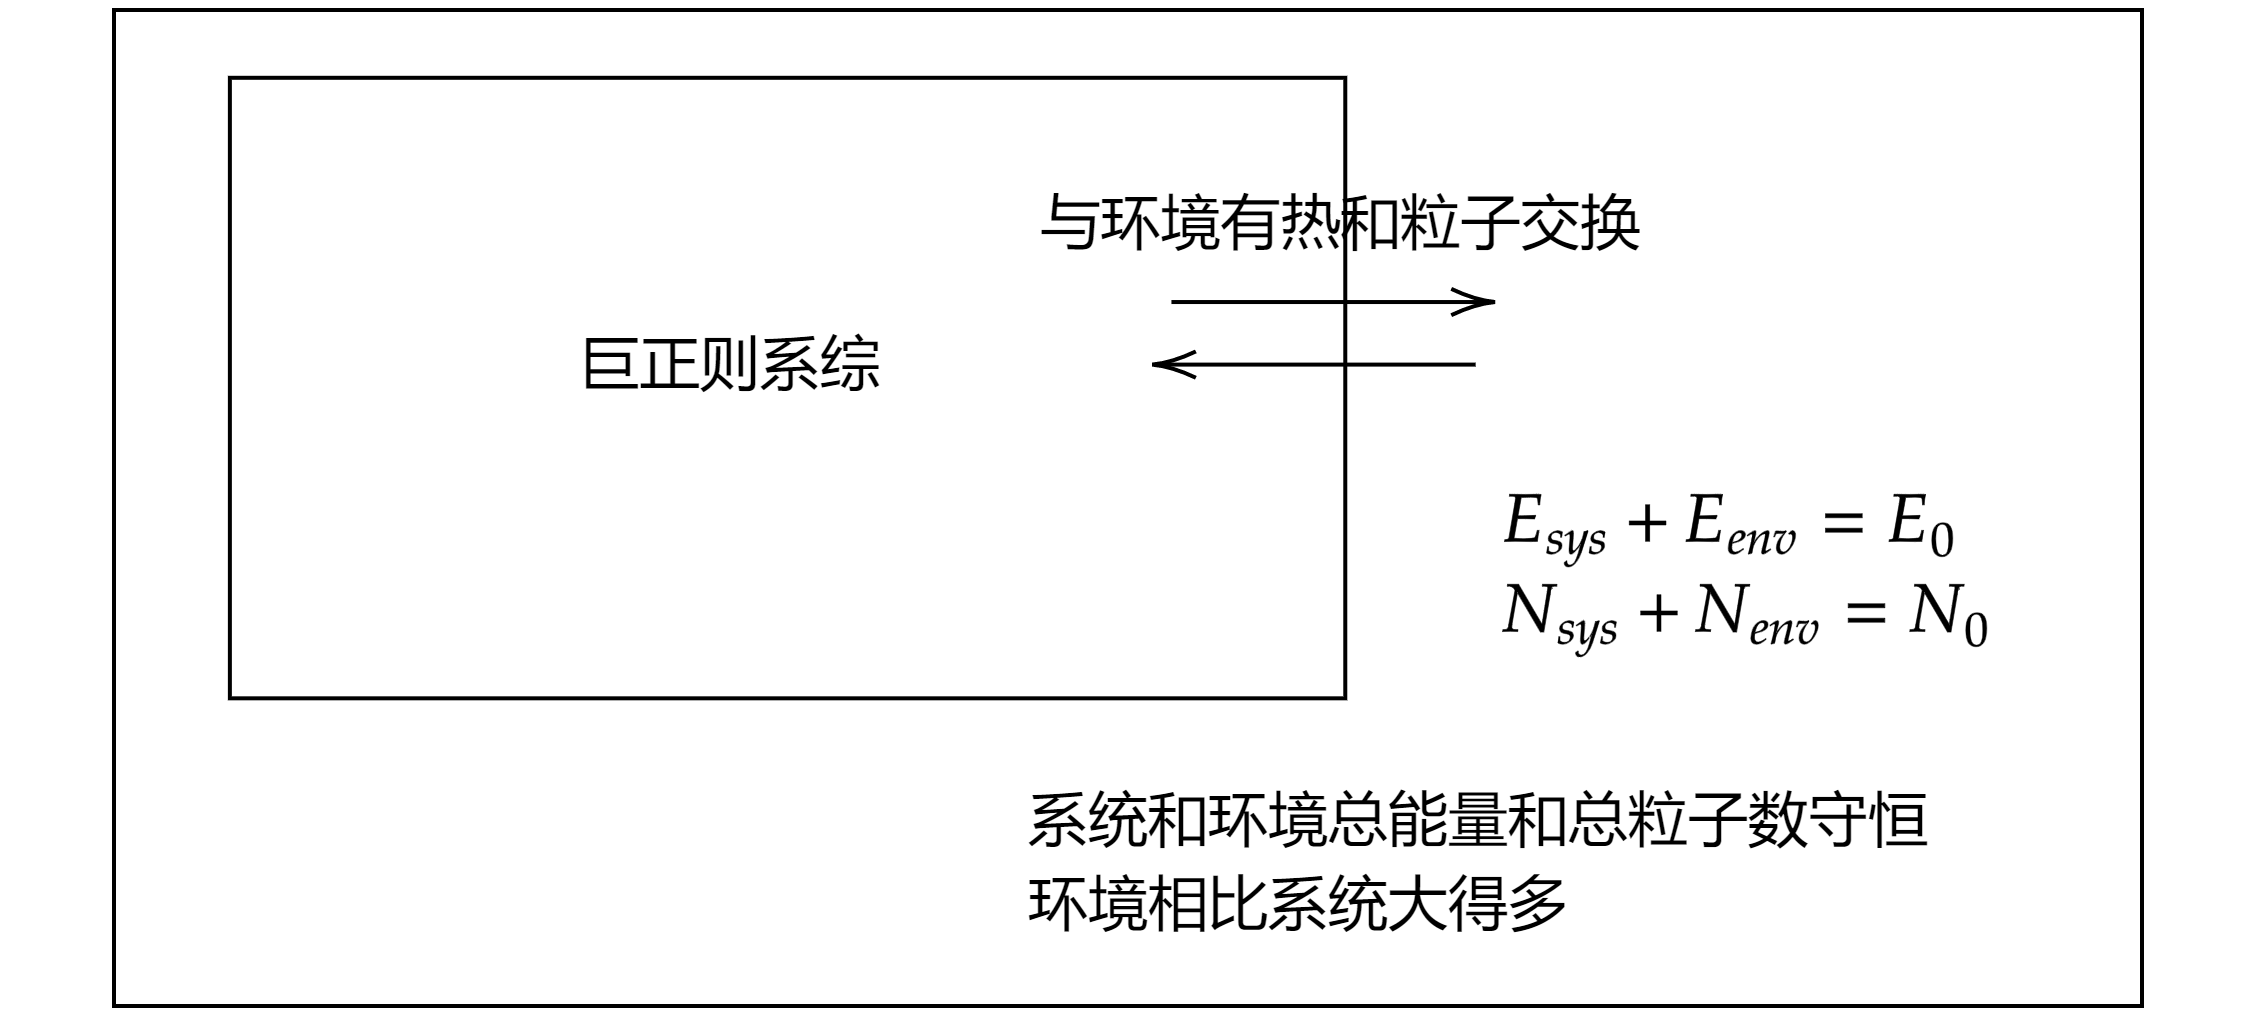
\includegraphics[width=0.6\textwidth]{fig/巨正则系综.png} 
      \caption{巨正则系综}
\end{figure}


和任一微观态的概率 $p_v$ 为\begin{equation}
       p_v=\frac{e^{-\beta E_v-\mu N_v}}{\Xi}
\end{equation}
其熵的表达式为\begin{equation}
       S=k_B (\ln \Xi+\beta E-\beta\mu N)=k_B \ln \Xi +\frac{E-\mu N}{T}
\end{equation}

从其熵的表达式我们不难得到\begin{equation}
       k_B T\ln \xi =TS -E+\mu N=-A+G =pV
\end{equation}
即$pV=k_BT \ln \Xi$,因此就有\begin{equation}
       \di (pV)=p\di V+V\di p=k_B T \di \ln \Xi+k_B\ln \xi \di T
\end{equation}
我们已知系统的$\mu,V,T$,利用$\ln \Xi$可以直接求出\begin{align}
       E&=\braket{E}=-\diffp*{\ln \Xi}{\beta}{\zeta, V}\\
       N&=\braket{N}=-\diffp*{\ln \Xi}{{(-\beta\mu)}}{\beta,V}\\
       S&=k_B \ln \Xi +\frac{E-\mu N}{T}\\
\end{align}
为了求出其他热力学量,我们利用\begin{equation}
       \di \ln \Xi =\beta p \di V+\beta V\di p -k_B \beta \ln \Xi \di T 
\end{equation}
而\begin{equation}
       \di G=\mu \di N+N\di \mu=V\di p -S\di T +\mu \di N
\end{equation}
所以$V\di p =S\di T +N\di \mu $,于是有\begin{equation}
       \di \ln \Xi =\beta p \di V+\beta (S-K_B \ln \Xi)\di T +\beta N \di \mu
\end{equation}
进而有\begin{equation}
       p=k_B T \diffp*{\ln \Xi}{V}{\mu,T}
\end{equation}

接下来我们讨论$E$和$N$的涨落,在正则系综中,我们有结论\begin{equation}
       \braket{(\Delta E)^2}=kT^2 \diffp{\braket{E}}{T}=kT^2 C_V
\end{equation}
对于$N$的涨落,我们有\begin{equation}
       \braket{(\Delta N)^2}=\diffp*{\braket{N}}{{(\beta\mu)}}{\beta,V}=kT \diffp*{\braket{N}}{\mu}{V,T}
\end{equation}

由数学结论\begin{equation}
       \diffp*{x}{y}{z} \diffp*{y}{z}{x}\diffp*{z}{x}{y}=-1
\end{equation}

所以就有\begin{equation}
       \diffp*{N}{\mu}{V,T}\cdot \diffp*{\mu}{V}{N,T}\cdot \diffp*{V}{N}{\mu,T}=-1
\end{equation}
所以\begin{equation}
       \diffp*{N}{\mu}{V,T}=-\diffp*{V}{\mu}{N,T}\cdot \diffp*{N}{V}{\mu,T}
\end{equation}
注意到\begin{equation}
       \di G=V\di p -S\di T +\mu \di N=\mu \di N+N\di \mu
\end{equation}
所以就有 \begin{equation}
       N\di \mu=V\di p-S\di T
\end{equation}
因此有Maxwell关系\begin{equation}
    \diffp{\mu}{p}=\diffp{V}{N}   
\end{equation}
以及\begin{equation}
       \diffp*{\mu}{p}{T}=\frac{V}{N}
\end{equation}
因此\begin{equation}
       \diffp*{V}{N}{T,\mu}=\frac{V}{N}
\end{equation}
所以\begin{equation}
       \diffp*{N}{\mu}{V,T}=-\frac{N}{V}\diffp*{V}{\mu}{N,T}=-\frac{N}{V} \left(\diffp{V}{p}\diffp{p}{\mu}\right)_{N,T}=-\frac{N^2}{V^2} \diffp*{p}{V}{N,T}=\frac{N^2}{V}\kappa
\end{equation}
其中\begin{equation}
       \kappa=\frac{1}{V}\diffp*{p}{V}{N,T}
\end{equation}
我们称为体变模量\index{体变模量}。所以\begin{equation}
       \braket{(\Delta N)^2}=kT \diffp*{\braket{N}}{\mu}{V,T}=\frac{kTN^2\kappa}{V}
\end{equation}
% subsection 巨正则系综的热力学关系 (end)
\subsubsection{$N$的巨正则分布} % (fold)
\label{ssub:N的巨正则分布}
因为任意微观态的概率为
\begin{equation}
       p_v=\frac{1}{\displaystyle \Xi} \exp\left(-\frac{E_v-\mu N_v}{kT}\right)
\end{equation}
并且\begin{equation}
       N_v=N_v(E_v,V)
\end{equation}
所以\begin{equation}
       p(N_v=N)=\sum_{v,\,N_v=N} p_v=\frac{e^{\beta\mu N}}{\displaystyle \Xi} \sum_{v,\,N_v=N} e^{-\beta E_v(N,v)} =\frac{e^{\beta\mu N}}{\displaystyle \Xi} Q(N,V,T)
\end{equation}
因此\begin{equation}
       \ln p(N) =\beta\mu N -\ln \Xi(\mu,V,T) +\ln Q(N,V,T)
\end{equation}
对$\ln p(N)$在$\braket{N}$附近做Taylor展开,可以得到\begin{equation}
       \ln p(N) =\ln p(\braket{N})+\left.\diffp{\ln p(\braket{N})}{N}\right|_{\braket{N}}(N-\braket{N}) +\left.\frac{1}{2}\diffp[2]{\ln p(\braket{N})}{N}\right|_{\braket{N}} (N-\braket{N})^2 +o(N^2)
\end{equation}

考虑到\begin{equation}
       \diffp{\ln p(N)}{N}=\beta \mu +\diffp*{\ln Q}{N}{V,T}=\beta\mu-\beta\mu=0
\end{equation}
而\begin{equation}
       \diffp[2]{\ln p(N)}{N}=\diffp*{\ln Q}{{N^2}}{V,T}
\end{equation}
因此\begin{equation}
       \left.\frac{1}{2}\diffp[2]{\ln p(\braket{N})}{N}\right|_{\braket{N}}=\diffp{{-\beta \mu }}{{\langle N\rangle} }=-\frac{1}{\braket{(\Delta N)^2}}
\end{equation}
也即\begin{equation}
       \ln p(N)= \ln p(\braket{N})-\frac{1}{2}\frac{(N-\braket{N})}{\braket{(\Delta N)^2}}
\end{equation}
因此$N$的概率分布为\begin{equation}
      p(N)=p(\braket{N})\exp\left(-\frac{(N-\braket{N})^2}{2\sigma_N^2}\right)
\end{equation}
% subsubsection $N$的巨正则分布 (end)
\subsubsection{热力学极限情形} % (fold)
\label{ssub:热力学极限情形}
考虑$N=\braket{N}$的时候\begin{equation}
       \Xi (\mu,V,T)=\sum_{v,\,N_v=\braket{N}} e^{-\beta E_v}=\sum_{v,\,N_v=\braket{N}} e^{-\beta E_v(\braket{N},v)}=e^{\beta\mu \braket{N}}Q(\braket{N},V,T)
\end{equation}
这个时候\begin{equation}
       k_BT \ln \Xi =pV =\mu N +k_BT \ln Q(\braket{N},V,T)=G-A
\end{equation}
是自洽的。
% subsubsection 热力学极限情形 (end)
% subsection 巨正则系综 (end)
\subsection{等温等压系综} % (fold)
\label{sub:等温等压系综}
等温等压系综的状态参量为$N,p,T$,有配分函数\begin{equation}
       \mathcal{Z}=(\beta p,N,\beta) =\sum_{v} e^{-\beta E_v-\beta pV_v}
\end{equation}
以及相对应的熵\begin{equation}
       S=k_B\ln \mathcal{Z} +\frac{E+pV}{T}
\end{equation}
核心热力学关系\begin{equation}
       k_BT\ln \mathcal{Z}=TS-E-pV=TS-H
\end{equation}
即\begin{equation}
       G=-k_B T\ln \mathcal{Z}
\end{equation}
其他的推导都是类似的,在这里就不赘述了

\begin{review}
       \item 正则系综的定义、状态参量;
       \item 配分函数的定义及其应用;
       \item 能量的涨落、正则分布;
       \item Sackur‐Tetrode 方程;
       \item Gibbs熵的定义;
       \item Gibbs熵和与Boltzman熵的联系;
       \item 广义系综的定义;
       \item 广义配分函数;
       \item 巨正则系综的定义;
       \item 粒子数的巨正则分布;
\end{review}
% subsection 等温等压系综 (end)
% section 广义系综 (end)
\section{习题} % (fold)
\label{sec:习题2}
\begin{enumerate}
       \item We know that the free energy  $F(T, V, N)$  of a thermodynamic system is extensive. Show that

       \[N\left(\frac{\partial F}{\partial N}\right)_{T, V}+V\left(\frac{\partial F}{\partial V}\right)_{T, N}=N f=F\]
       
       with  $f$  the free energy density expressed in suitable variables. Given this result, from the differential properties of  $F(T, V, N)$ , show that
       
       \[\Phi=N \mu\]
       
       with  $\Phi$  the Gibbs potential defined as $\Phi=F+P V $. In the above expression, $ \mu $ is the chemical potential properly defined in terms of $ F(T, V, N) $.
\end{enumerate}
% section 习题 (end)
% chapter 正则系综和广义系综 (end)